\documentclass[11pt,letterpaper]{article}
\pdfminorversion=7 % Match the PDF 1.7 vector figures exported from Gephi styling.

% Network Science Assignment 1 — editable report template.
% Compile from this directory using: pdflatex -interaction=nonstopmode -halt-on-error -output-directory=build main.tex
% Repeat once for references and table of contents, or run build_report.ps1.

\usepackage[margin=1in]{geometry}
\usepackage[T1]{fontenc}
\usepackage{lmodern}
\usepackage{microtype}
\usepackage{amsmath,amssymb}
\usepackage{booktabs,tabularx}
\usepackage{graphicx}
\usepackage{xcolor}
\usepackage{hyperref}
\hypersetup{colorlinks=true,linkcolor=blue!50!black,urlcolor=blue!50!black,citecolor=blue!50!black}
\graphicspath{{../results/plots/}{../results/gephi/}}

% Delete a \pending{...} line when the corresponding content is written.
\newcommand{\pending}[1]{\par\smallskip\begingroup\color{gray}\itshape\sloppy\noindent[To complete: #1]\par\endgroup\smallskip}
\newcommand{\missing}{\textemdash}

\title{\bfseries Assignment 1: Network Analysis and Visualization\\
  \large Frontiers of Network Science (CSCI 4250)}
\author{Student: [Your Name]\\Fall 2026}
\date{Due: October 23, 2026}

\begin{document}
\maketitle
\noindent\textbf{Submission:} PDF report plus reproducible code/supporting files via Submitty.\\
\noindent\textbf{Draft status:} Review draft for discussion; final revisions and submission approval are pending.
\tableofcontents
\clearpage

\section{Task 1: Real-World Network Description}
\subsection{Real-World Networks}

\subsubsection{General Relativity and Quantum Cosmology Collaboration Network (ca-GrQc)}

The General Relativity and Quantum Cosmology Collaboration Network (ca-GrQc) represents scientific collaborations among authors who submitted papers to the General Relativity and Quantum Cosmology (GR-QC) category of arXiv. The dataset covers submissions from January 1993 to April 2003 and is provided by the Stanford Network Analysis Project (SNAP)~\cite{snap-ca-grqc}.

Each node represents an author, and an undirected edge connects two authors who co-authored at least one paper. Papers with multiple authors form fully connected subgraphs (cliques). The network contains \textbf{5,242 nodes and 14,496 edges} and is undirected and unweighted, with multiple collaborations between the same authors represented by a single edge.

The network supports the study of research communities, clustering, and connectivity in scientific collaboration.

\subsubsection{Western States Power Grid}

The Western States Power Grid network represents the electrical transmission infrastructure of the western United States. It is available through Mark Newman's Network Data Collection~\cite{newman-power-grid} and was used in Watts and Strogatz's 1998 study of small-world networks~\cite{watts1998smallworld}.

Nodes represent generators, transformers, or substations, while edges represent transmission lines connecting these facilities. The network contains \textbf{4,941 nodes and 6,594 edges} and is undirected and unweighted. It describes the physical connectivity of the power grid without including transmission capacities or electricity-flow directions.

The network supports comparisons of connectivity, clustering, and path lengths between physical infrastructure and theoretical network models.

\begin{table}[htbp]
\centering
\caption{\textbf{Original dataset metadata.}}
\label{tab:dataset-metadata}
\begin{tabularx}{\linewidth}{@{}Xrrcc@{}}
\toprule
Network & Nodes & Edges & Directed? & Weighted? \\
\midrule
ca-GrQc & 5,242 & 14,496 & No & No \\
Western States Power Grid & 4,941 & 6,594 & No & No \\
\bottomrule
\end{tabularx}
\par\smallskip
\begin{minipage}{\linewidth}
\textit{Sources: SNAP~\cite{snap-ca-grqc} and Mark Newman's Network Data Collection~\cite{newman-power-grid}.}
\end{minipage}
\end{table}

\clearpage
\section{Network Generation: ER and BA Counterparts}

For each real network with $N$ nodes and $M$ edges, the Erd\H{o}s--R\'enyi (ER) model was generated using $p=2M/[N(N-1)]$. The Barab\'asi--Albert (BA) model used the integer attachment parameter $m$ giving the closest available edge count. All models used random seed 42. For ca-GrQc, 12 self-loops were removed from the analysis copy before setting the model parameters, leaving 5,242 nodes and 14,484 edges.

\begin{table}[!htbp]
\centering
\caption{\textbf{Reference-model parameters and generated graph sizes.}}
\label{tab:model-parameters}
\small
\begin{tabularx}{\linewidth}{@{}Xlrrrl@{}}
\toprule
Base network & Model & Nodes & Edges & Seed & Parameter \\
\midrule
ca-GrQc & ER & 5,242 & 14,176 & 42 & $p=0.001054405$ \\
ca-GrQc & BA & 5,242 & 15,717 & 42 & $m=3$ \\
Power Grid & ER & 4,941 & 6,431 & 42 & $p=0.000540303$ \\
Power Grid & BA & 4,941 & 4,940 & 42 & $m=1$ \\
\bottomrule
\end{tabularx}
\end{table}

The standard BA model could not closely match the Power Grid's 6,594 edges: $m=1$ produced 4,940 edges (25.08\% fewer), while $m=2$ would produce 9,878 edges. Thus, $m=1$ was selected as the closer option.

\section{Task 2: Global Network Properties}

Diameter, radius, and average eccentricity were calculated on the largest connected component (LCC) of each network. Connected-component counts and degree statistics were calculated over the full graph. Degree variance is the population variance ($\mathrm{ddof}=0$).

\begin{table}[!htbp]
\centering
\caption{\textbf{Network sizes and connectivity (full graph).}}
\label{tab:global-connectivity}
\small
\begin{tabularx}{\linewidth}{@{}Xrrrr@{}}
\toprule
Network & Nodes & Edges & Components & LCC nodes \\
\midrule
ca-GrQc (real) & 5,242 & 14,484 & 355 & 4,158 \\
ca-GrQc (ER) & 5,242 & 14,176 & 19 & 5,223 \\
ca-GrQc (BA) & 5,242 & 15,717 & 1 & 5,242 \\
Power Grid (real) & 4,941 & 6,594 & 1 & 4,941 \\
Power Grid (ER) & 4,941 & 6,431 & 387 & 4,504 \\
Power Grid (BA) & 4,941 & 4,940 & 1 & 4,941 \\
\bottomrule
\end{tabularx}
\end{table}

\begin{table}[!htbp]
\centering
\caption{\textbf{Distance measures (LCC) and degree statistics (full graph).}}
\label{tab:global-distances}
\small
\setlength{\tabcolsep}{4pt}
\begin{tabularx}{\linewidth}{@{}Xrrrrr@{}}
\toprule
Network & Diameter & Radius & \shortstack[r]{Mean\\eccentricity} & Mean degree & \shortstack[r]{Degree\\variance} \\
\midrule
ca-GrQc (real) & 17 & 9 & 11.675 & 5.526 & 62.690 \\
ca-GrQc (ER) & 10 & 7 & 8.047 & 5.409 & 5.157 \\
ca-GrQc (BA) & 7 & 4 & 5.686 & 5.997 & 74.714 \\
Power Grid (real) & 46 & 23 & 34.541 & 2.669 & 3.209 \\
Power Grid (ER) & 20 & 12 & 14.924 & 2.603 & 2.465 \\
Power Grid (BA) & 20 & 10 & 14.390 & 2.000 & 16.740 \\
\bottomrule
\end{tabularx}
\end{table}

The real ca-GrQc network has 355 components and a diameter of 17, compared with 19 components and a diameter of 10 for ER, and one component and a diameter of 7 for BA. Its degree variance (62.690) is substantially greater than ER's (5.157).

The real Power Grid is connected and has a diameter of 46, while its ER counterpart has 387 components and a diameter of 20 on its LCC. Both reference models have substantially smaller mean eccentricities than the real Power Grid.

\clearpage
\section{Task 3: Network Distributions}
\begingroup
\setlength{\emergencystretch}{1em}
\setlength{\textfloatsep}{8pt}
\setlength{\intextsep}{7pt}

Four distributions are reported for each network. Degree and local clustering use all nodes; eccentricity uses exact Task 2 results on the LCC; component size uses one observation per component, including the LCC. Table~\ref{tab:distribution-summary} gives means and population variances ($\mathrm{ddof}=0$), calculated from original observations. Probabilities are normalized by the relevant sample size. Logarithmic axes are used where appropriate; degree plots preserve zero using a symmetric logarithmic horizontal scale. Clustering uses 20 equal-width interior bins and separate zero/one masses. Curves are descriptive, not significance tests; detailed fitting settings are documented in the supporting reproduction guide.

\begin{table}[!htbp]
\centering
\caption{\textbf{Distribution means and population variances.} Eccentricity uses LCC nodes; clustering uses all nodes; component size uses one observation per component, including the LCC.}
\label{tab:distribution-summary}
\small
\setlength{\tabcolsep}{3pt}
\begin{tabularx}{\linewidth}{@{}Xrrrrrr@{}}
\toprule
& \multicolumn{2}{c}{Eccentricity} & \multicolumn{2}{c}{Local clustering} & \multicolumn{2}{c}{Component size} \\
\cmidrule(lr){2-3}\cmidrule(lr){4-5}\cmidrule(l){6-7}
Network & Mean & Variance & Mean & Variance & Mean & Variance \\
\midrule
ca-GrQc (real) & 11.675 & 1.204 & 0.529636 & 0.183768 & 14.766 & 48,495.396 \\
ca-GrQc (ER) & 8.047 & 0.206 & 0.000921 & 0.000092 & 275.895 & 1,359,658.410 \\
ca-GrQc (BA) & 5.686 & 0.227 & 0.009484 & 0.002331 & 5,242.000 & 0 \\
Power Grid (real) & 34.541 & 13.827 & 0.080104 & 0.050260 & 4,941.000 & 0 \\
Power Grid (ER) & 14.924 & 1.153 & 0.000502 & 0.000281 & 12.767 & 52,257.104 \\
Power Grid (BA) & 14.390 & 2.701 & 0 & 0 & 4,941.000 & 0 \\
\bottomrule
\end{tabularx}
\end{table}

\clearpage

\subsection{Degree Distribution}
Figures~\ref{fig:degree-grqc} and~\ref{fig:degree-power} show empirical degree probabilities. Real-network curves use shifted negative-binomial fits with a separate zero mass; ER curves use $\mathrm{Binomial}(N-1,p)$ references. BA curves fit discrete power-law tails only, scaled by the empirical tail fraction. These fits do not establish a power-law hypothesis~\cite{clauset2009powerlaw}. Degree means and variances appear in Table~\ref{tab:global-distances}.

\begin{figure}[!htbp]
\centering\small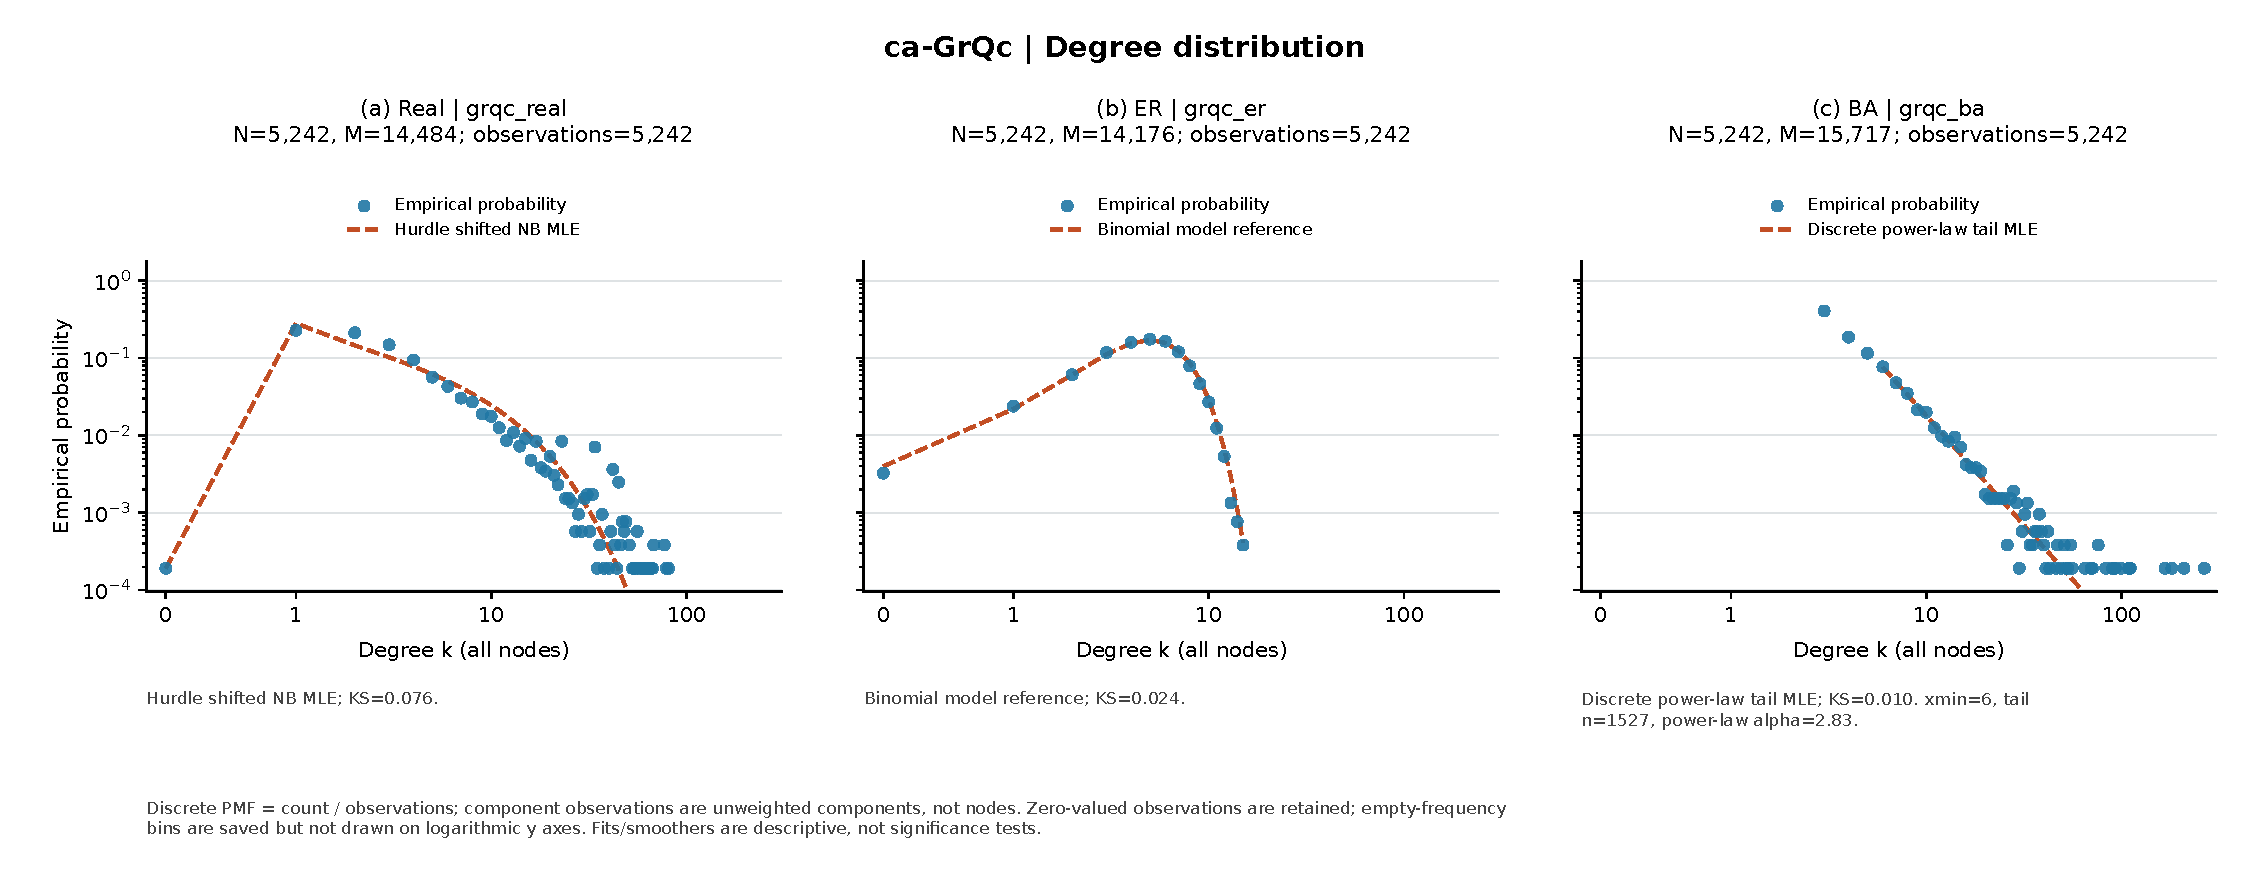
\includegraphics[width=0.96\linewidth]{task3/grqc__degree.pdf}
\caption{\textbf{Degree distributions for ca-GrQc and its ER/BA counterparts.} All nodes are included. Dashed curves show the real-network count fit, ER reference, and BA tail fit, respectively.}
\label{fig:degree-grqc}
\end{figure}
\begin{figure}[!htbp]
\centering\small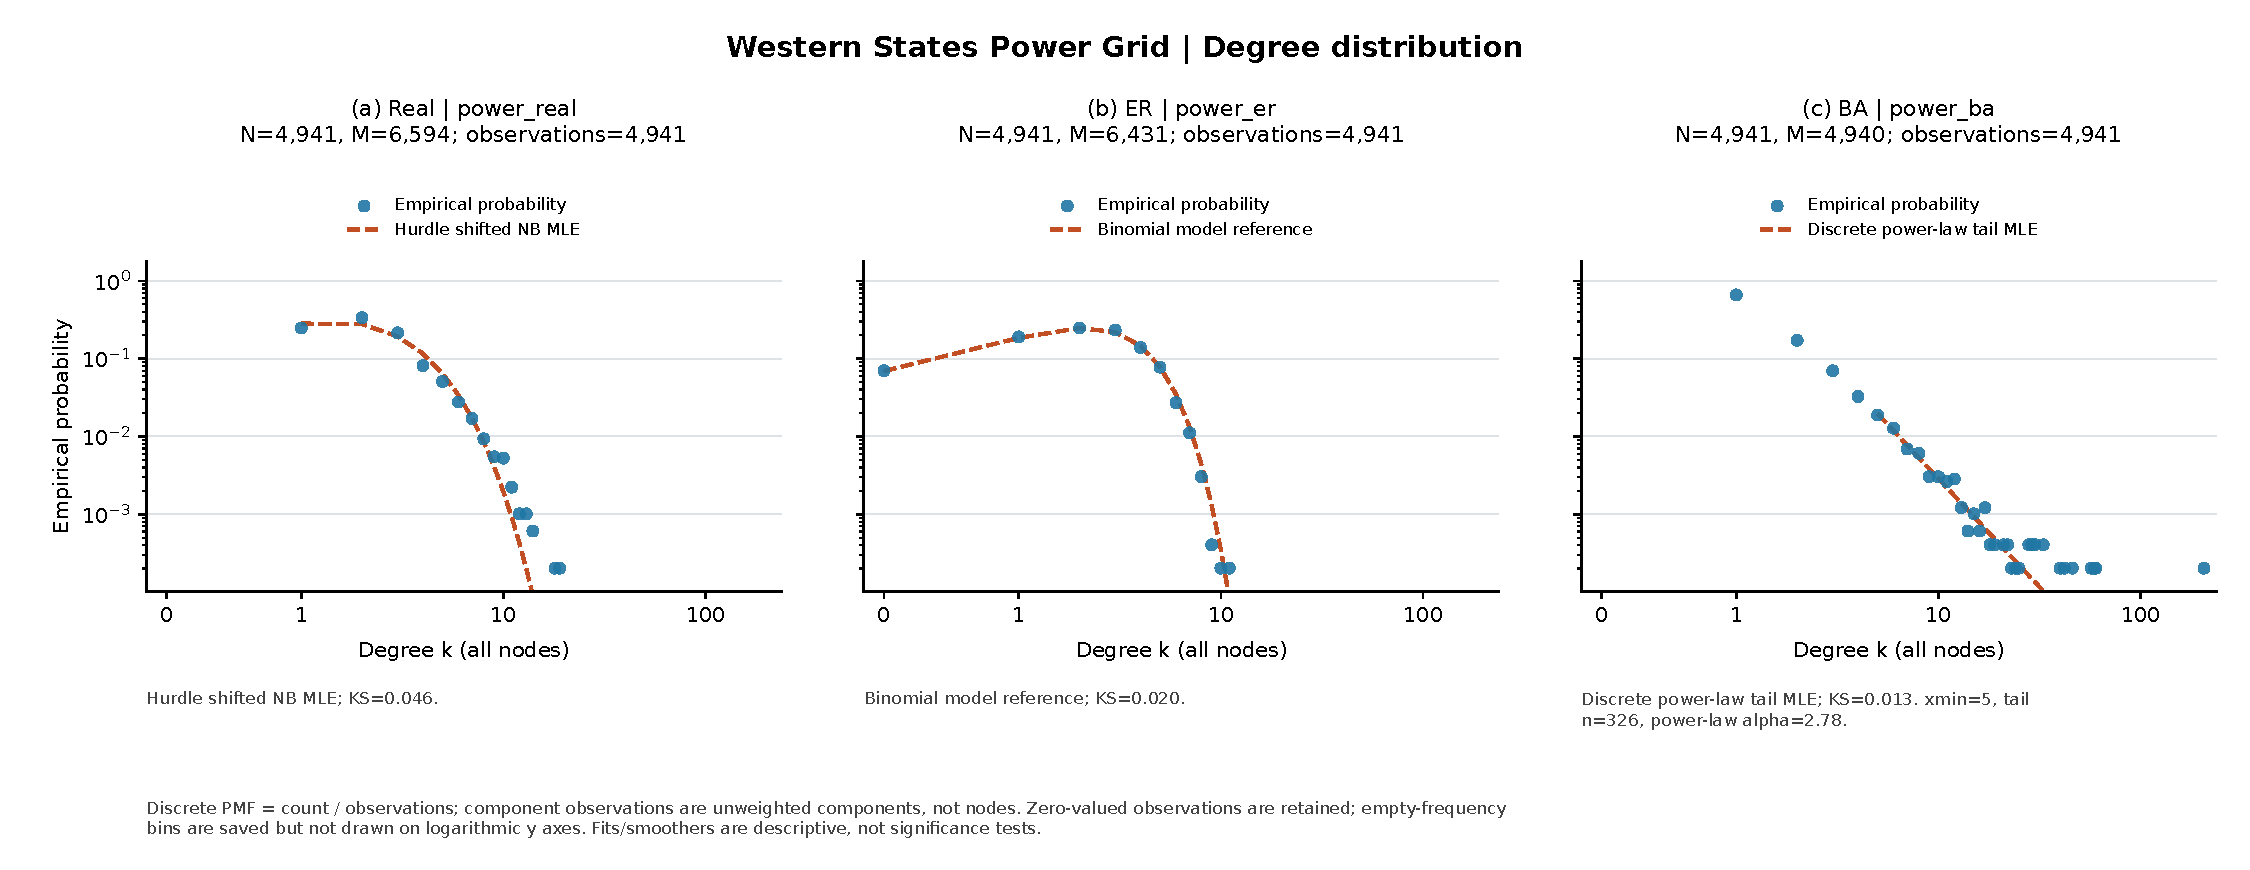
\includegraphics[width=0.96\linewidth]{task3/power__degree.pdf}
\caption{\textbf{Degree distributions for Power Grid and its ER/BA counterparts.} The BA curve describes degrees $k\geq5$ only; the full empirical distribution is retained.}
\label{fig:degree-power}
\end{figure}
\clearpage

\subsection{Longest-Shortest-Path (Eccentricity) Distribution}
Eccentricity is $e(v)=\max_{u\in\mathrm{LCC}}d(v,u)$, measured in hops. Figures~\ref{fig:ecc-grqc} and~\ref{fig:ecc-power} use one observation per LCC node. Curves are bounded discrete-normal fits, except for Power Grid BA, which uses a beta-binomial fit. All curves are restricted to the observed integer support from radius to diameter.

\begin{figure}[!htbp]
\centering\small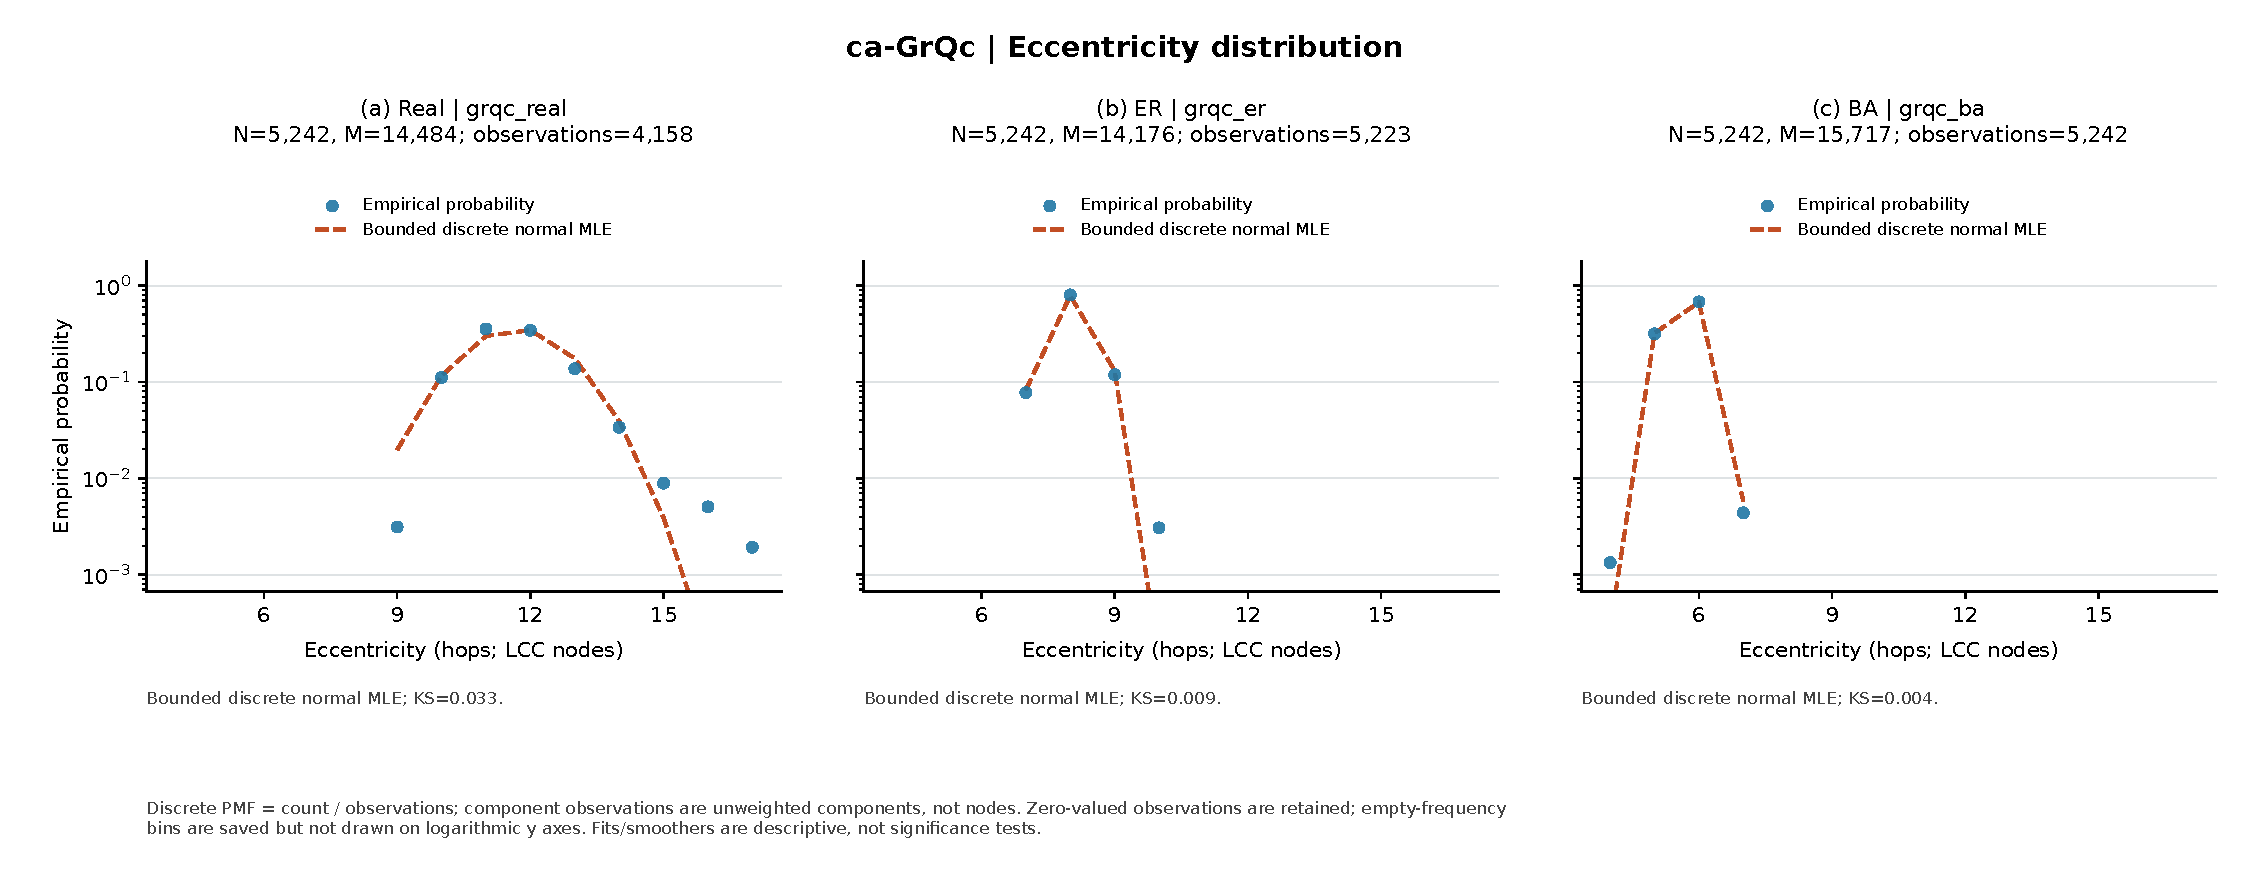
\includegraphics[width=0.96\linewidth]{task3/grqc__eccentricity.pdf}
\caption{\textbf{Eccentricity distributions for ca-GrQc and its ER/BA counterparts.} Each observation is an LCC node. Dashed curves are bounded discrete-normal fits on the observed integer supports.}
\label{fig:ecc-grqc}
\end{figure}
\begin{figure}[!htbp]
\centering\small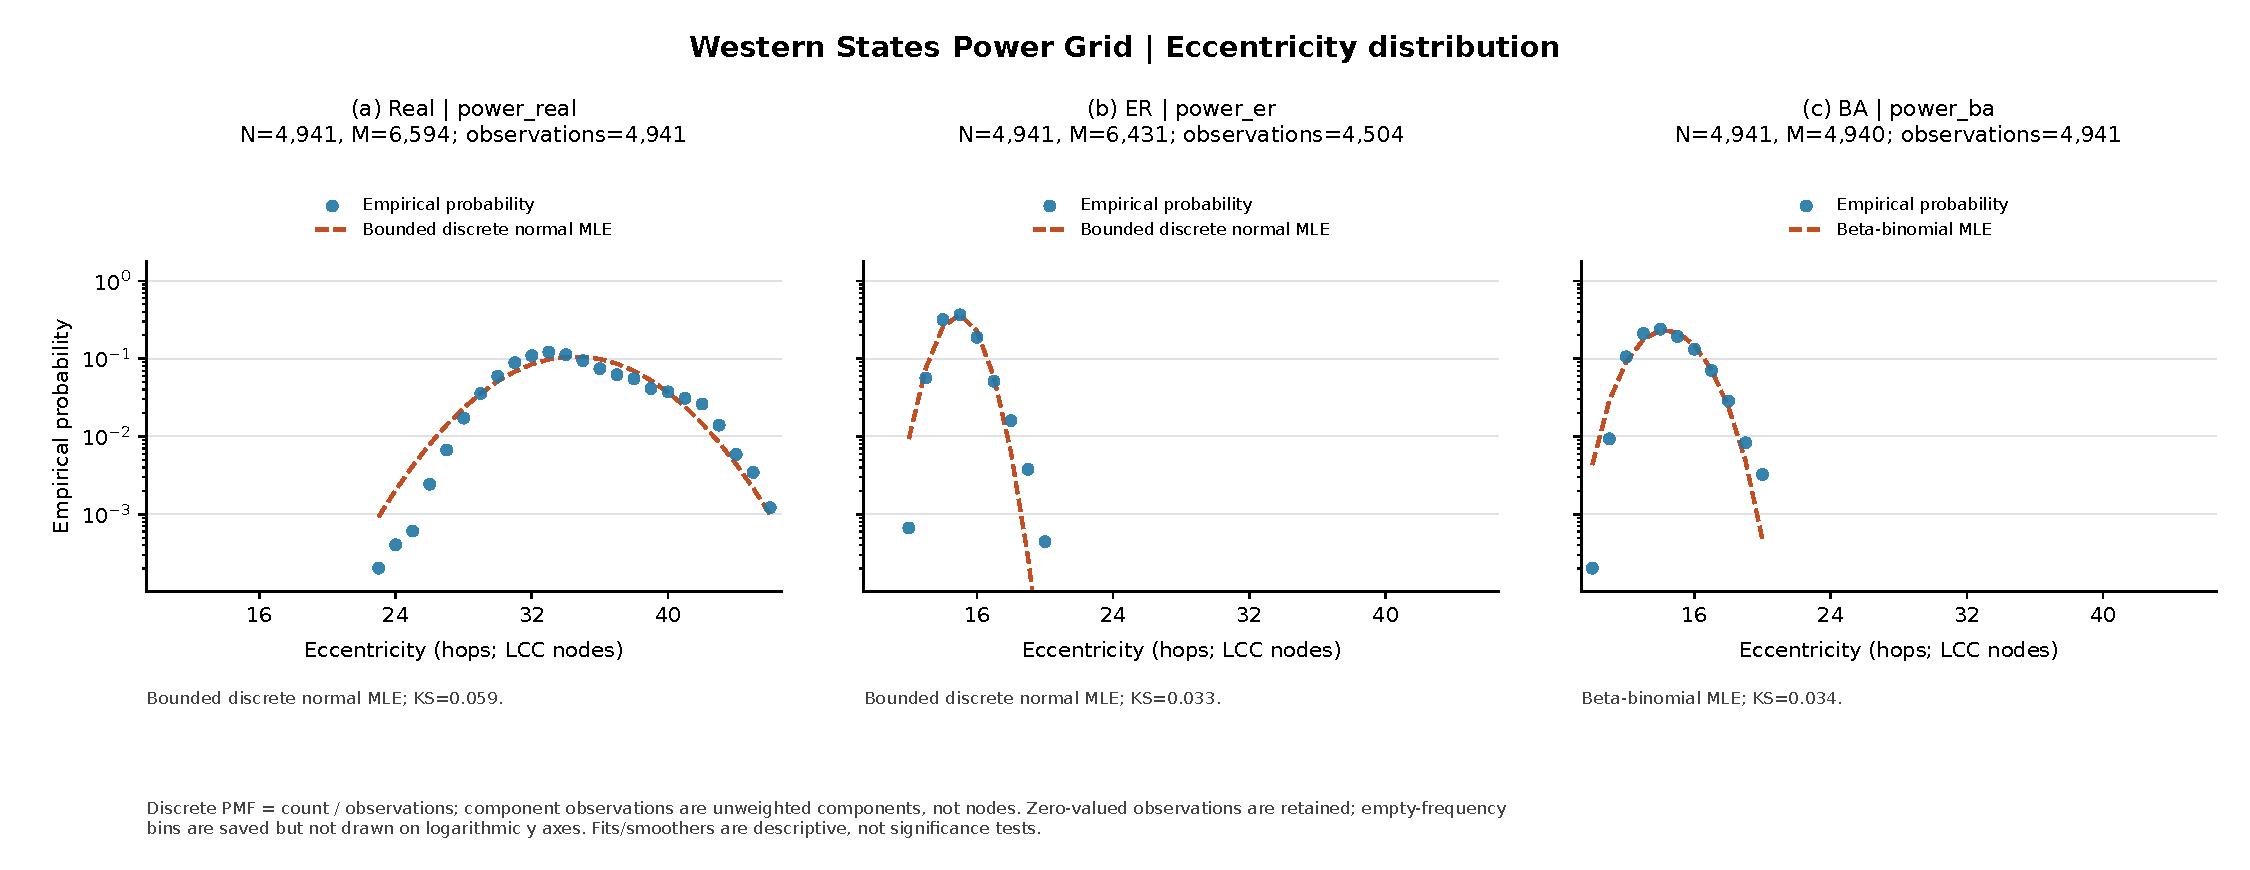
\includegraphics[width=0.96\linewidth]{task3/power__eccentricity.pdf}
\caption{\textbf{Eccentricity distributions for Power Grid and its ER/BA counterparts.} Curves are bounded discrete-normal fits for real/ER and a beta-binomial fit for BA. Distances are in hops.}
\label{fig:ecc-power}
\end{figure}
\clearpage

\subsection{Clustering-Coefficient Distribution}
Figures~\ref{fig:clustering-grqc} and~\ref{fig:clustering-power} include all nodes, assigning zero to degree-zero/one nodes. Four curves use reflected kernel density estimation (KDE), integrated over bins, as descriptive smoothers after Beta fits failed the selected screen. Continuous fits are N/A for Power Grid ER (eight interior observations) and BA (all-zero clustering because $m=1$ produces a tree).

\begin{figure}[!htbp]
\centering\small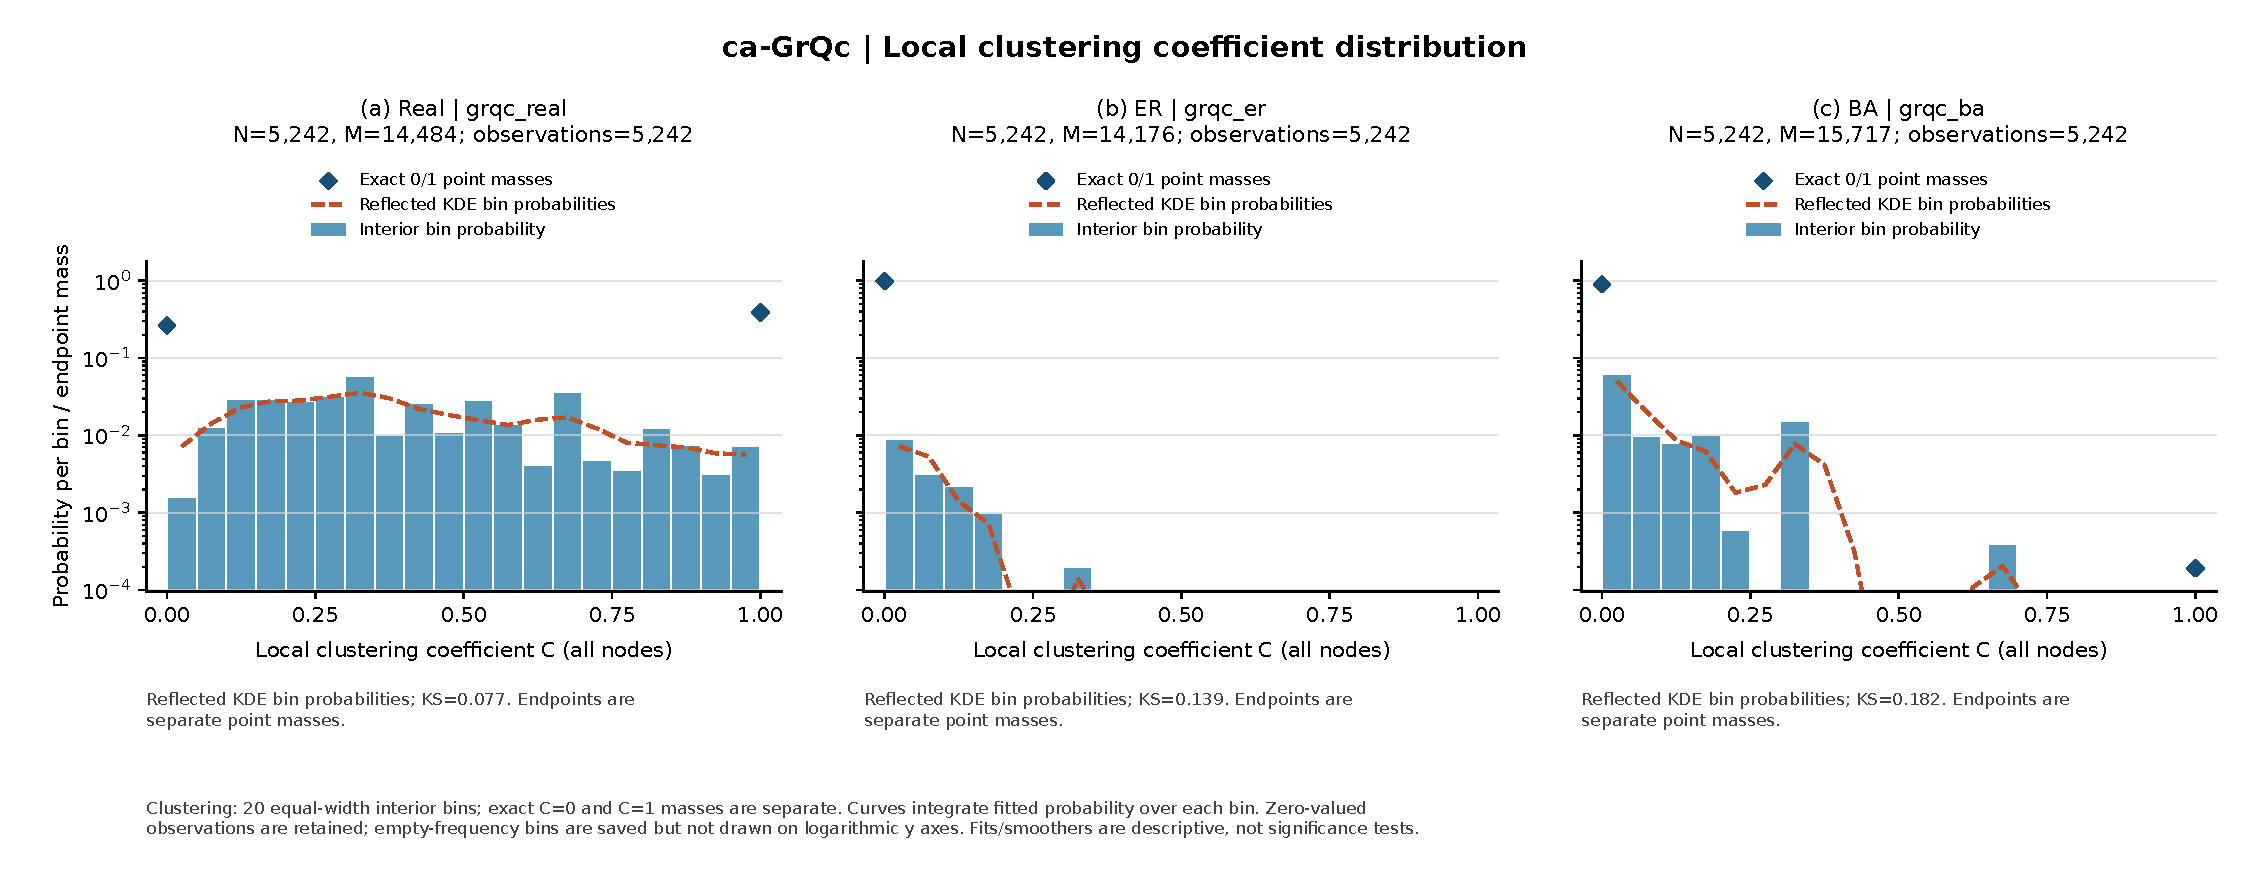
\includegraphics[width=0.96\linewidth]{task3/grqc__clustering.pdf}
\caption{\textbf{Local clustering distributions for ca-GrQc and its ER/BA counterparts.} Bars show interior probabilities, diamonds show endpoint masses, and dashed curves show KDE bin probabilities.}
\label{fig:clustering-grqc}
\end{figure}
\begin{figure}[!htbp]
\centering\small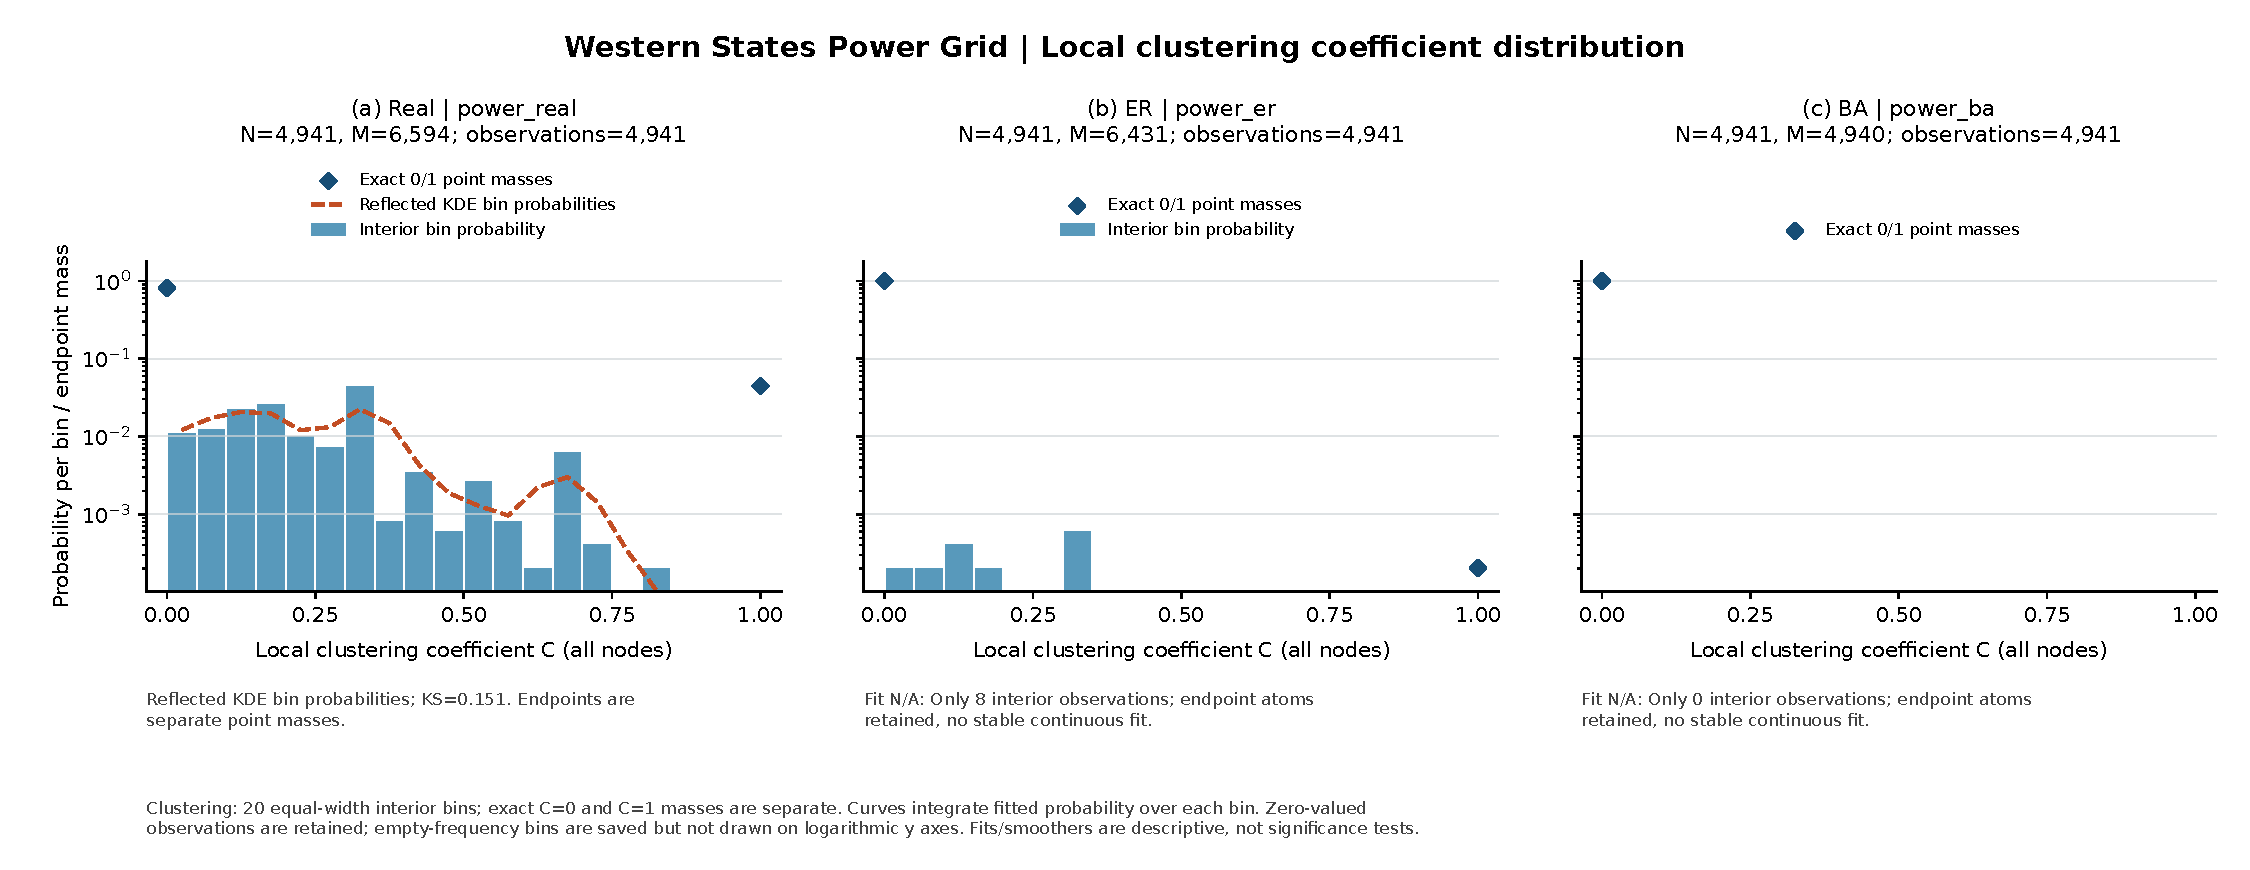
\includegraphics[width=0.96\linewidth]{task3/power__clustering.pdf}
\caption{\textbf{Local clustering distributions for Power Grid and its ER/BA counterparts.} The real-network curve is a KDE smoother. ER/BA fits are N/A; all nodes are included.}
\label{fig:clustering-power}
\end{figure}
\clearpage

\subsection{Connected-Component Size Distribution}
Figures~\ref{fig:components-grqc} and~\ref{fig:components-power} weight components equally. Power Grid ER fits non-LCC sizes with a shifted negative binomial, scaled by their component fraction. Fits are N/A for connected graphs (one observation), real ca-GrQc (failed fit screen), and ca-GrQc ER (18 non-LCC observations). The latter two follow the chosen fitting policy. All moments include the LCC.

\begin{figure}[!htbp]
\centering\small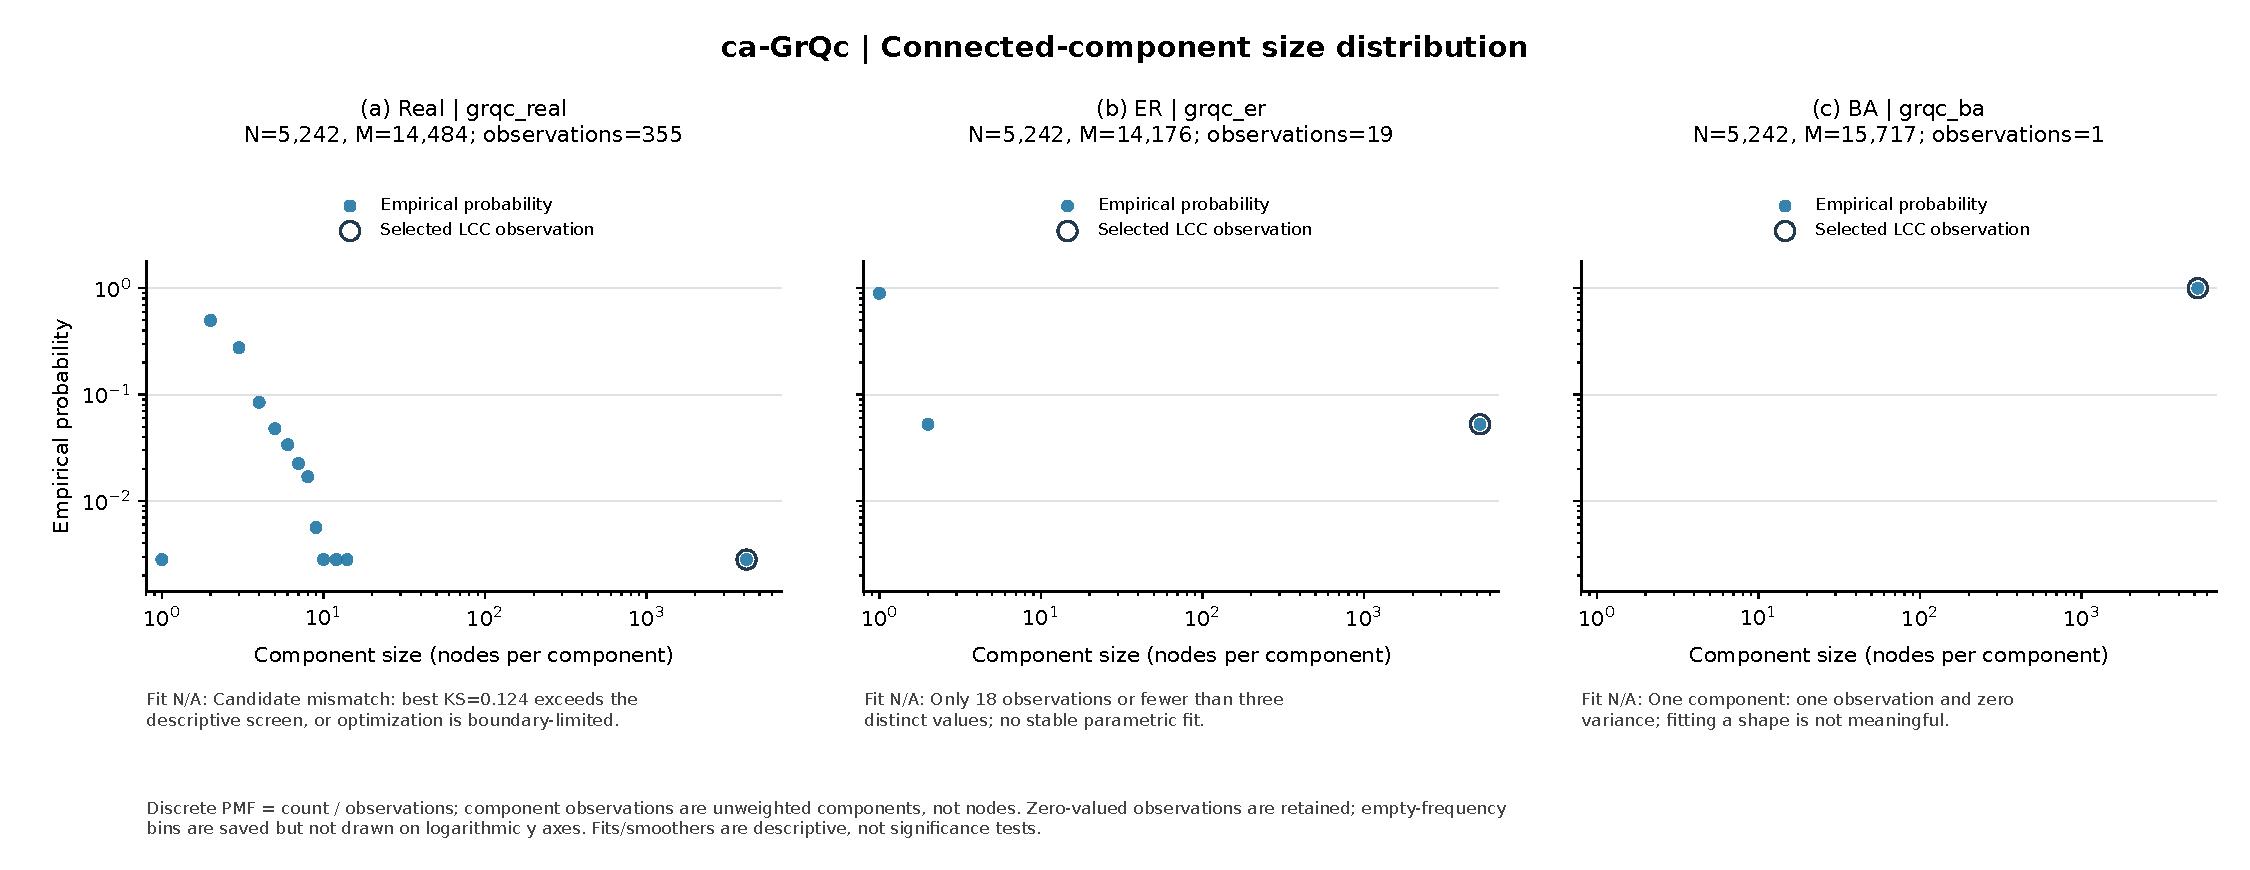
\includegraphics[width=0.96\linewidth]{task3/grqc__component_size.pdf}
\caption{\textbf{Component-size distributions for ca-GrQc and its ER/BA counterparts.} Probabilities are per component, not per node. All components are shown; N/A annotations explain the omitted curves.}
\label{fig:components-grqc}
\end{figure}
\begin{figure}[!htbp]
\centering\small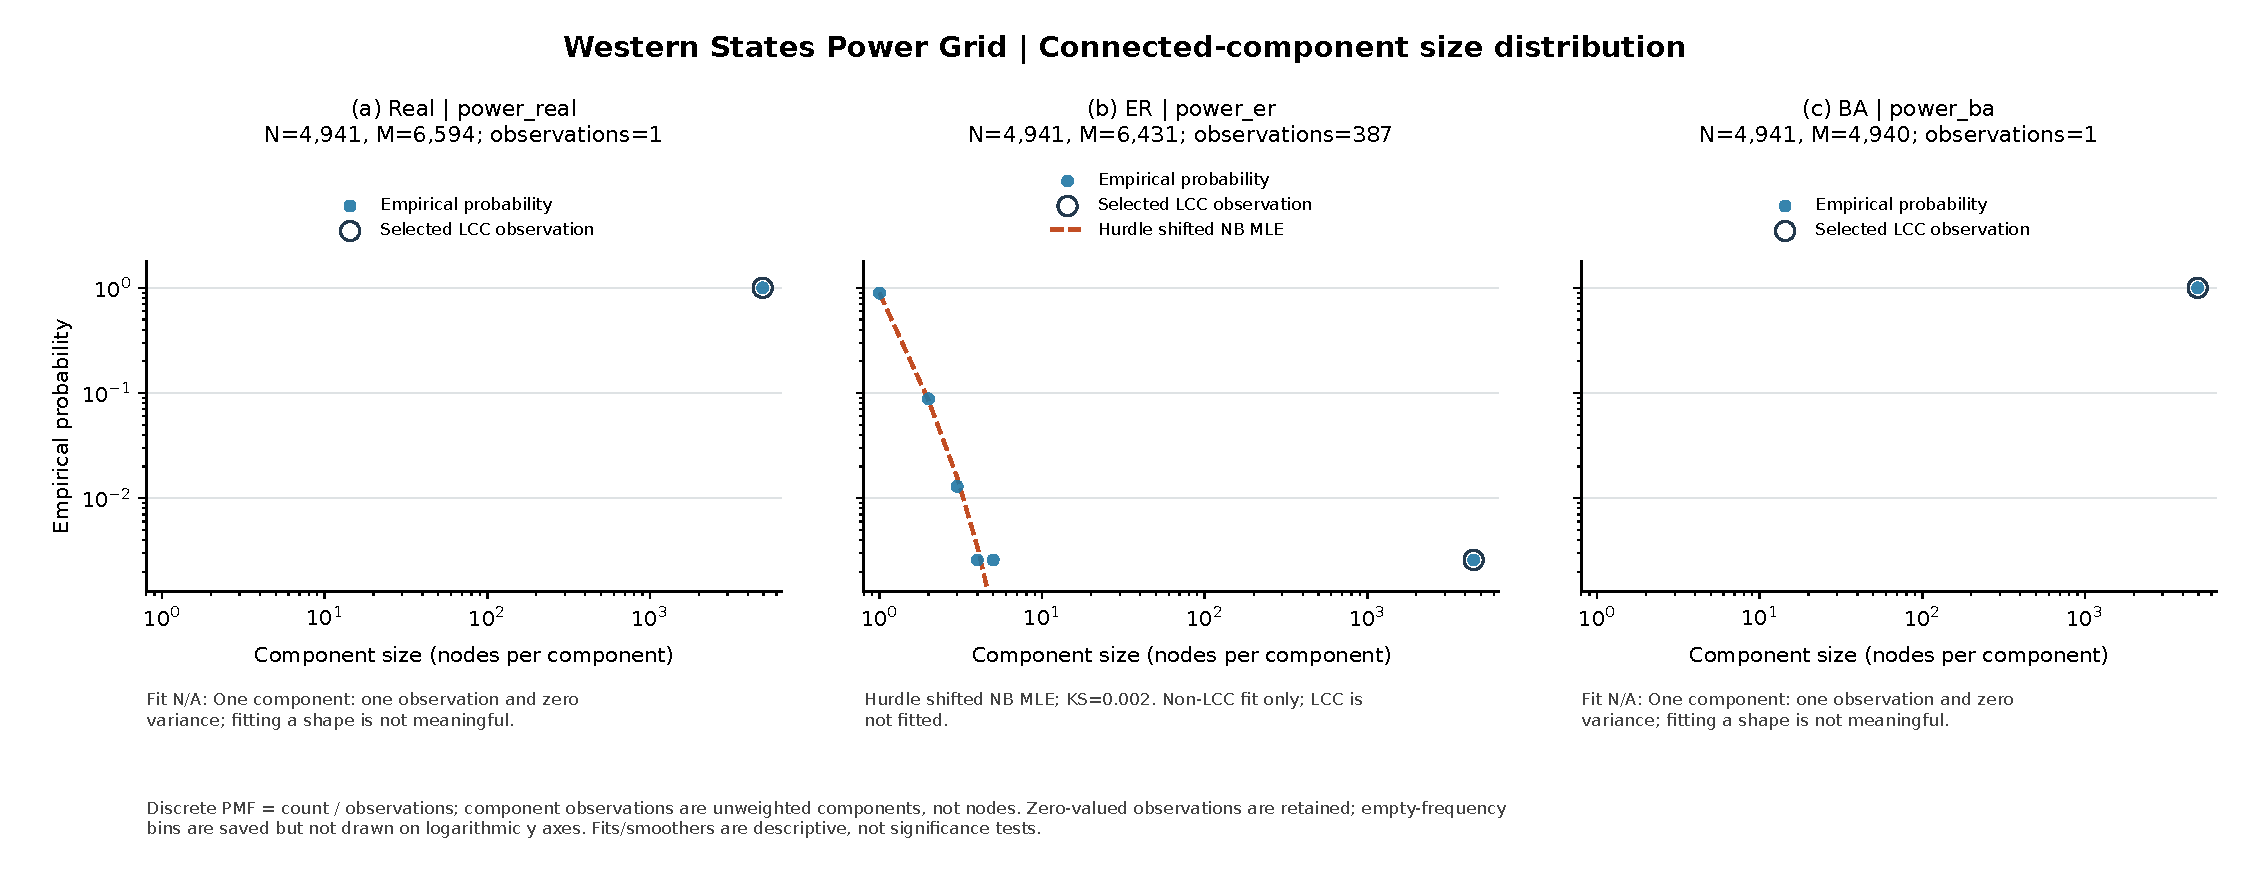
\includegraphics[width=0.96\linewidth]{task3/power__component_size.pdf}
\caption{\textbf{Component-size distributions for Power Grid and its ER/BA counterparts.} The ER curve fits non-LCC components only; the LCC and single-component real/BA graphs remain empirical observations.}
\label{fig:components-power}
\end{figure}
\clearpage
\endgroup

\section{Task 4: Comparison and Interpretation}

\subsection{ca-GrQc: Real vs ER vs BA}
The real ca-GrQc network has substantially greater degree heterogeneity than ER: their degree variances are 62.690 and 5.157, respectively (Table~\ref{tab:global-distances}). BA is closer on this measure, with variance 74.714, but its maximum degree of 266 exceeds the real network's 81 (Figure~\ref{fig:degree-grqc}). Thus, preferential attachment provides a more suitable description of unequal connectivity than independent random edges in this comparison, without reproducing the full observed degree distribution or establishing how the real network formed.

Neither model captures the strong local clustering. Mean clustering is 0.529636 in the real network, compared with 0.000921 for ER and 0.009484 for BA (Table~\ref{tab:distribution-summary}; Figure~\ref{fig:clustering-grqc}). The high real-network clustering is consistent with its construction: coauthors of a multi-author paper form a clique. Neither reference model explicitly includes this group-based construction.

The models also underrepresent fragmentation and LCC distances. The real graph has 355 components, versus 19 for ER and one for BA (Table~\ref{tab:global-connectivity}; Figure~\ref{fig:components-grqc}). Mean eccentricity is 11.675 in the real LCC, versus 8.047 and 5.686, respectively (Figure~\ref{fig:ecc-grqc}). These differences indicate that matching node counts and approximate edge counts does not reproduce component structure or distances within the largest component. BA captures degree heterogeneity more closely, but neither model jointly reproduces clustering, fragmentation, and eccentricity.

\subsection{Western States Power Grid: Real vs ER vs BA}
ER is closer to the Power Grid's degree variability: its variance is 2.465, compared with 3.209 for the real graph and 16.740 for BA (Table~\ref{tab:global-distances}). Maximum degrees are 11, 19, and 206 for ER, real, and BA, respectively (Figure~\ref{fig:degree-power}). BA therefore introduces much stronger hub dominance than observed, whereas ER better approximates the relatively narrow degree distribution.

This agreement does not extend to connectivity or distances. The real grid is connected, while ER has 387 components, including 345 isolates; BA is connected (Table~\ref{tab:global-connectivity}; Figure~\ref{fig:components-power}). Nevertheless, both models have much smaller mean eccentricities: 14.924 for ER and 14.390 for BA, versus 34.541 for the real grid (Figure~\ref{fig:ecc-power}). ER distances describe only its LCC. The real grid's longer distances are consistent with geographically constrained infrastructure, although these measurements do not establish that explanation causally.

Mean clustering is 0.080104 in the real grid, 0.000502 in ER, and zero in BA (Figure~\ref{fig:clustering-power}). BA's zero clustering follows from its $m=1$ tree construction. Its 25.08\% edge deficit (Table~\ref{tab:model-parameters}) also confounds structural comparisons, so differences cannot be attributed solely to attachment rules. ER better approximates degree variability and BA preserves connectedness, but neither reproduces the grid's clustering and eccentricity. Across both datasets, conclusions concern single seeded realizations with unequal realized edge counts, not ensemble-level model performance.
\clearpage

\section{Task 5: Methodology and Reproducibility}

\subsection{Data Sources and Preprocessing}
The original ca-GrQc edge list was obtained from SNAP~\cite{snap-ca-grqc}, and Power Grid from Newman's collection~\cite{newman-power-grid}. Raw archives and extracted files are preserved under \path{data/raw/}. The ca-GrQc input is \path{data/raw/ca-GrQc.txt/CA-GrQc.txt}; Power Grid uses \path{data/raw/power/power.gml}. Input SHA-256 checksums, archive-integrity checks, parsing diagnostics, and original sizes are recorded in the input-audit files under \path{results/tables/}.

ca-GrQc was read as a two-column integer edge list, ignoring comment and blank lines. Malformed records were checked; none were found. Reciprocal records were combined into single undirected edges without assigning weights. Its original 5,242 nodes and 14,496 edges include 12 self-loops. Only these loops were removed from the analysis copy, leaving 5,242 nodes and 14,484 edges. All vertices were retained, including node 12295, which became isolated. Power Grid was read from GML with \texttt{label=None}, preserving declared numeric node IDs. It contains no self-loops or duplicate edges, and remains at 4,941 nodes and 6,594 edges. Neither network required weight removal, imputation, or additional filtering. Both were analyzed as simple, undirected, unweighted graphs; the edge-list format cannot reveal any unlisted upstream isolates.

The LCC is the component containing the most nodes, with ties resolved by the smallest numeric node ID. Only distance-based measures use its induced subgraph; degree, clustering, and component statistics retain the full graph.

\subsection{Generation Settings}
Each reference model uses the analyzed real network's node count. ER uses \texttt{gnp\_random\_graph} with $p=2M/[N(N-1)]$, calculated without pre-rounding, so $M$ is the expected rather than enforced edge count. BA uses \texttt{barabasi\_albert\_graph} with the default initial star. Its integer $m$ minimizes $|m(N-m)-M|$, choosing the smaller $m$ if tied. No edges were adjusted after generation. All four samples use seed 42; Table~\ref{tab:model-parameters} records parameters and realized sizes. Full-precision settings and edge-count differences are saved in \path{task2_config.json} and \path{results/tables/task2_model_parameters.csv}.

\subsection{Software and Computation}
Analysis used Python 3.12.15 in Conda environment \texttt{fons-a1}: NetworkX 3.7 for graphs, generation and clustering; NumPy 2.5.4 for moments; pandas 2.3.3 for tabular checks; SciPy 1.18.1 for fitting; Matplotlib 3.11.2 for figures; and pytest 9.1.1 for validation. The report was compiled with MiKTeX-pdfTeX 4.27 (MiKTeX 26.5), with automatic package installation and shell execution disabled.

Exact unweighted breadth-first search was performed once per LCC node. The resulting eccentricities determine diameter, radius, and mean eccentricity and are cached for Task 3; no distance approximation was used. All variances use \texttt{ddof=0}. Clustering includes degree-zero/one nodes with coefficient zero; component-size observations are equally weighted components. Checks include degree sum $2M$, component-size sum $N$, LCC bounds, finite moments, deterministic model generation, and agreement between tables and cached observations. The latest independent verification passed all 55 tests.

Fits are descriptive: maximum-likelihood candidates are compared by AIC on a common sample, with a chosen KS-distance screen of 0.10 rather than a significance test. ER degree references retain the generation probability; BA degree fits use discrete power-law tails, compared with lognormal alternatives. Eccentricity candidates use observed integer bounds. Clustering retains exact zero/one masses and uses reflected Gaussian KDE with Scott bandwidth when Beta fits fail the screen. Component fits exclude the LCC, require at least 50 observations and three distinct sizes, and are scaled by the non-LCC fraction; all reported moments still include the LCC. Failed, sparse, or degenerate fits are labeled N/A. Candidate diagnostics, parameters, and limitations are retained in \path{task3_config.json}, the fit tables, and \path{TASK3_REPRODUCIBILITY.md}.

Matplotlib uses the non-interactive Agg backend. Eight three-panel composites cover all 24 distributions, with shared scales within each comparison. Figures are exported as vector PDF and 200-dpi PNG; numerical samples, probabilities, and clustering bins are saved separately. Regenerated figures require renewed visual review.

\subsection{Reproduction Instructions}
Use the original inputs at the paths above and the recorded package versions. From the project root, run the following PowerShell commands. The Conda path is specific to the verified workstation and may be replaced with the corresponding local installation. A project-local temporary directory avoids pytest access conflicts.

\begingroup\footnotesize
\begin{verbatim}
& .\scripts\preflight.ps1
$cx = 'C:\ProgramData\anaconda3\Scripts\conda.exe'
$env:TEMP = Join-Path $PWD 'results/cache/reproduction_tmp'
$env:TMP = $env:TEMP
New-Item -ItemType Directory -Force $env:TEMP | Out-Null
& $cx run -n fons-a1 --no-capture-output python `
  src/run_task2.py
& $cx run -n fons-a1 --no-capture-output python `
  scripts/refresh_task2_manifest.py --write
& $cx run -n fons-a1 --no-capture-output python `
  src/run_task3.py
& $cx run -n fons-a1 --no-capture-output python `
  src/run_task3.py --verify-only
& .\report\build_report.ps1
\end{verbatim}
\endgroup

Task 2 audits the inputs, applies preprocessing, generates models, and computes or reuses validated exact caches. The manifest-refresh utility validates the six saved graphs, caches and numerical tables before updating the output checksums required by Task 3; it preserves the previous manifest. Task 3 then computes distributions, fits and figures without regenerating models or shortest paths. Verify before rebuilding the report: saved provenance includes the report state at calculation time. After a report edit, regenerate Task 3 outputs to record the new state before using its verification mode; do not silently relabel stale provenance. To reproduce only Task 3 from unchanged Task 2 outputs, omit the Task 2 and manifest-refresh commands.

The reproducibility materials comprise \path{src/}, \path{scripts/}, \path{tests/}, both configuration files, \path{environment.yml}, \path{requirements.txt}, and the two task-specific reproduction guides. Include the source/audit metadata, six processed GraphML files, required caches, numerical CSV/JSON files, figures, and LaTeX sources with the supporting materials. Caches are Git-ignored locally, so a supplement must include them explicitly or regenerate them. The dependency file gives compatible ranges; the exact versions above and machine-readable version records identify the analyzed environment. Numerical tables retain full precision; report rounding is for presentation only.

\section{Optional: Real-World Network Visualizations}

\subsection{ca-GrQc Visualization}
\pending{Insert a high-quality SVG/PDF-derived figure for ca-GrQc, explain the node/edge visual encodings, filtering choices, layout, legend, and export settings.}

\subsection{Western States Power Grid Visualization}
\pending{Insert the power-grid network visualization; document decluttering, layout, sizes/colors/labels, legend, and why the representation is appropriate.}

% Delete this section's \input line from main.tex if you decide not to submit the bonus.

\clearpage
\begin{thebibliography}{9}
\bibitem{snap-ca-grqc}
Stanford Network Analysis Project (SNAP),
\emph{General Relativity and Quantum Cosmology collaboration network (ca-GrQc)}.
\url{https://snap.stanford.edu/data/ca-GrQc.html}.
Accessed October 17, 2026.

\bibitem{leskovec2007graph}
J.~Leskovec, J.~Kleinberg, and C.~Faloutsos,
``Graph evolution: Densification and shrinking diameters,''
\emph{ACM Transactions on Knowledge Discovery from Data}, vol.~1, no.~1,
Article~2, 41 pages, 2007.
\url{https://doi.org/10.1145/1217299.1217301}.

\bibitem{newman-power-grid}
M.~E.~J. Newman,
\emph{Network data: power grid of the western United States}.
\url{https://public.websites.umich.edu/~mejn/netdata/}.
Power Grid entry and accompanying \texttt{power.zip} documentation.
Accessed October 17, 2026.

\bibitem{watts1998smallworld}
D.~J.~Watts and S.~H.~Strogatz,
``Collective dynamics of `small-world' networks,''
\emph{Nature}, vol.~393, pp.~440--442, 1998.
\url{https://doi.org/10.1038/30918}.
\bibitem{clauset2009powerlaw}
A.~Clauset, C.~R.~Shalizi, and M.~E.~J. Newman,
``Power-law distributions in empirical data,''
\emph{SIAM Review}, vol.~51, no.~4, pp.~661--703, 2009.
\url{https://doi.org/10.1137/070710111}.
\end{thebibliography}


\end{document}
